\documentclass[12pt]{article}
\usepackage[margin=0.75in]{geometry}
\usepackage{indentfirst}
\usepackage{tikz}
\usepackage{pgfplots}

\title{\bf Money and Banking - Assignment 1}
\author{Kaitlin Poskaitis, Joshua Matthews, Ryan Couch, Emma Magaw}
\date{}

\begin{document}

\maketitle

%Question 1
\section{What is a bond's yield to maturity if it has a \$1000 face value and a
coupon rate of 10\%? The bond is currently selling for \$1,044.98 and has 2 
years to maturity.}

$$P = \frac{C}{1+i} + \frac{C}{(1+i)^2}$$

Where C = Coupon payment, F = Face value, P = Price, and i = Yield to maturity

$$1044.98 = \frac{100}{1 + i} + \frac{100}{(1 + i)^2}$$

$$i = 7.495\%$$


%Question 2
\section{What is the yield to maturity on a \$1,000-face value discount bond
maturing in one year that sells for \$800?}

$$i = \frac{F - P}{P}$$

Where F = Face value, i = Yield to maturity, and P = Current price

$$i = \frac{200}{800}$$

$$i = 25\%$$


%Question 3
\section{Explain why would you be more or less willing to buy an Apple bond in
the following situations:}

{\bf a.} Your wealth increases.

You would be more likely to buy an Apple bond because when your wealth 
increases, you will want to purchase more assets. A bond would fall under this 
category, so you will likely be more willing to buy an Apple bond.

{\bf b.} The US Treasury bonds become more liquid.

You would be less likely to buy an Apple bond in this case because the Apple
bond becomes less liquid than the US Treasury bonds, and the demand for an 
asset is positively related to its liquidity relative to other assets, so
you would be less willing to buy an Apple bond as a result.

{\bf c.} Expect gold to appreciate in value.

You would be less likely to buy an Apple bond because, assuming gold is a 
substitute for the Apple bond, the demand for gold would increase and, as a
result, the demand for the Apple bond will decrease since gold is anticipated
to appreciate in value.

%Question 4
\section{Using the supply and demand for bonds framework show what the effect is
on interest rates when the riskiness of bonds rises. Use appropriate supply and
demand diagrams.}

\pgfplotsset{
	every axis/.append style={extra description/.code={
		\node at (0.87,0.80) {$S_1$};
		\node at (0.87,0.20) {$D_1$};}
	}
}
\centerline{
\begin{tikzpicture}
	\begin{axis}[xtick=\empty,ytick=\empty,xlabel=Quantity,ylabel=Price]
		\addplot[domain=0:10, mark=none, smooth, blue] {x};
		%\addlegendentry{Supply}
		\addplot[domain=0:10, mark=none, smooth, red] {-x+10};
		%\addlegendentry{Demand}
		%\addplot[mark=none, samples=100, red] function{x};
		%\addplot[mark=none, samples=100, blue] function {-x};
	\end{axis}
\end{tikzpicture}
}


\pgfplotsset{
	every axis/.append style={extra description/.code={
		\node at (0.87,0.80) {$S_1$};
		\node at (0.87,0.20) {$D_1$};
		\node at (0.70,0.20) {$D_2$};}
	}
}

\vspace{5mm}

\centerline{
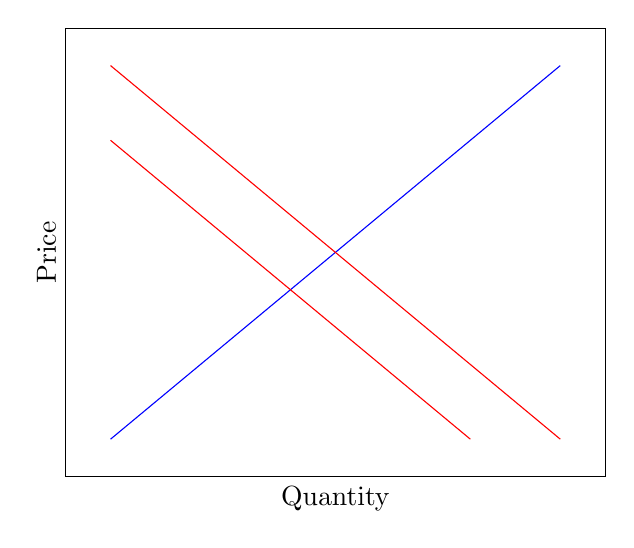
\begin{tikzpicture}
	\begin{axis}[xtick=\empty,ytick=\empty,xlabel=Quantity,ylabel=Price]
		\addplot[domain=0:10, mark=none, smooth, blue] {x};
		%\addlegendentry{Supply}
		\addplot[domain=0:10, mark=none, smooth, red] {-x+10};
		\addplot[domain=0:8, mark=none, smooth, red] {-x+8};
		%\addlegendentry{Demand}
		%\addplot[mark=none, samples=100, red] function{x};
		%\addplot[mark=none, samples=100, blue] function {-x};
	\end{axis}
\end{tikzpicture}
}

%Question 5
\section{Suppose there are 2 kinds of bonds- default free Treasury bonds and
corporate bonds. Risk premium on corporate bonds are usually anticyclical; 
that is, they decrease during business cycle expansions and increase during
recessions. Why is this so?}

As the economy goes into a period of expansion, companies are expected
to be more successful. Fewer companies will go bankrupt, and there is
expected to be less default risk. Expected default rates will become
lower, and credit spreads will become more narrow. As the economy goes
into a recession, the expected default rates will become higher and credit
spreads will become wider. Therefore, risk premiums on corporate bonds
will increase.  Therefore, risk premiums on corporate bonds are
anti-cyclical - they decrease during a business cycle of expansion, and
increase during a business cycle of recession.

%Question 6
\section{Suppose that income tax rates on the return on US Treasury bonds are
reduced such that the latter's after-tax expected return relative to municipal
bonds become greater. What effect would this have on the price and hence 
interest rates of municipal bonds?}

If the income tax rates on the return on US Treasury bonds are reduced such that
their after-tax expected return relative to municipal bonds becomes greater,
then the demand for municipal bonds will fall as they depreciate against the US
Treasure bonds. This lowered demand will lower the price, and therefore raise
the interest rate of the municipal bonds.

%Question 7
\section{Compute the price of a stock that pays \$1 per year dividend and that
you expect to be able to sell in one year for \$20, assuming you require a 
15\% return.}

$$P = \frac{D + P1}{1 + R}$$

Where P = Price of stock, D = Dividend, P1 = Expected price, and R = Expected 
return.

$$P = \frac{1 + 20}{1 + 0.15}$$ 
$$P = \frac{21}{1.15}$$ 
$$P = \$18.26$$

%Question 8
\section{If a corporation is expected to lose \$5 per share this year and it
actually loses \$4, what does the efficient market hypothesis say will happen 
to the price of stock when the actual loss is announced?}

The efficient market hypothesis states that in an efficient market, a
security's price fully reflects all publicly available information and
that all unexpected profit opportunities will be eliminated. Therefore, if
a stock's price is expected to drop \$5 and it is later announced that it
only dropped \$4, the price of that stock will then rise. The expected loss
was greater than the actual loss, so the price reflects upon this.

\end{document}
